\documentclass[a4paper,10pt]{article}

% Fancy maths stuff
\usepackage{amsmath, amsthm, amssymb}
%\usepackage{fullpage}

% Algorithm typesetting environments
\usepackage{algorithm}
\usepackage{algorithmic}

% Multi line tables
\usepackage{array}
\usepackage{booktabs}

%\usepackage{fullpage}

% Trees
\usepackage{qtree}

\usepackage{subfigure}

% Images
\usepackage{graphicx}

\begin{document}

% TITELPAGINA

\begin{titlepage}
\begin{center}

\vspace{2.5cm}

% [CHANGE] The title of your thesis. If your thesis has a subtitle, then this
% should appear right below the main title, in a smaller font.
\begin{Huge}
Performance Rendering using Structure Level Expression
\end{Huge}

\vspace{1.5cm}

% [CHANGE] Your full name. In case of multiple names, you can include their
% initials as well, e.g. "Jan G.J. van der Wegge".
Bastiaan J. van der Weij\\
% [CHANGE] Your student ID, as this has been assigned to you by the UvA
% administration.
5922151

\vspace{1.5cm}

% [DO NOT CHANGE]
Bachelor thesis\\
% [CHANGE] Whether your Bachelor thesis is 6 ECTS (regular) or 9 ECTS (Honours
% programme).
Credits: 15 EC

\vspace{0.5cm}

% [DO NOT CHANGE] The name of the educational programme.
Bachelor Opleiding Kunstmatige Intelligentie

\vspace{0.25cm}

% [DO NOT CHANGE] The address of the educational programme.
University of Amsterdam\\
Faculty of Science\\
Science Park 904\\
1098 XH Amsterdam

\vspace{4cm}

\emph{Supervisor}\\
% [CHANGE] The name of your supervisor. Include the titles of your supervisor,
% as well as the initials for *all* of his/her first names.
Prof. dr. ir. R.J.H. Scha

\vspace{0.25cm}

% [CHANGE] The address of the institute at which your supervisor is working.
% Be sure to include (1) institute (is appropriate), (2) faculty (if
% appropriate), (3) organization name, (4) organization address (2 lines).
Institute for Language and Logic\\
Faculty of Science\\
University of Amsterdam\\
Science Park 904\\
1098 XH  Amsterdam

\vspace{1.5cm}

% [CHANGE] The date at which you will finalize and submit your thesis.
June 24th, 2010

\end{center}

\end{titlepage}



\begin{abstract}
Both machine learning and rule based techniques have been extensively applied to performance rendering. However, relatively few systems make explicit use of machine learning combined with musical structure. Systems that use machine learning usually learn expression at note level. This paper introduces a performance rendering system that learns expression exclusively at a structural level. The system can be seen as complementary to systems that learn expression at note level. 

%Musical structure is extracted automatically. A dataset containing performances aligned to scores is then used to learn how structure relates to expression. A hidden Markov model is used to model this relation. Finally, the system can be applied to a a new score to produce an expressive performance. 


%This paper introduces a system for expressively performing transcribed music (scores) using statistical learning from a dataset. The dataset that is used contains performances aligned to the corresponding score. Expression is considered to be the way in which the performance deviates from the score. Expressive actions are predicted from links found between musical structure and expression. Previous expressive actions are also incorporated in the predictions. Musical structure will be automatically extracted from the scores using a set of formal rules that assign a hierarchical grouping structure to the music. To system will be able to deal with polyphonic music by splitting the scores into melody and harmony.

{\bf Keywords:} performance rendering, musical structure, constituent structure
\end{abstract}
\section{Introduction}

In the Western art music tradition it is customary that composers write down their compositions as scores. The task of a performer is to some extent to accurately reproduce the score; however, a perfect reproduction of a score generally sounds robotic and unpleasant. What makes a performance appealing is that the performer deviates from the score, altering timing, articulation and loudness, creating an expressive performance.

Given a hypothetical perfect synthesizer, performing scores with computers is a trivial task. However, \textit{expressively} performing music is not, and much research has focussed on this issue. A wide selection of scientific fields may have interest in such research: Artificial intelligence, cognitive science and musicology all benefit from a better understanding of expression in music. 

%Such systems Computers are widely used in music production. Since support for automatic expression is mostly absent or very poor in music editing software, some genres of music have evolved to sound acceptable even without expression. If good working automatic expression was available in software, computer music production could greatly widen its field of application.

A rather practical approach to expressive music performance is to recreate it. A performance rendering system is a computer program that automatically creates an expressive, human-like performance of a musical score. Performance rendering systems have always faced a problem of evaluation. It is debatable how much we should value correlation of generated performances with human performances of the same piece. A Chopin interpretation by Arthur Rubinstein can be radically different from a Chopin interpretation by Vladimir Horowitz, yet both are considered high quality interpretations. This problem has been one of the motivations for a yearly performance rendering event where performance rendering systems compete and are judged by an audience \cite{hiraga2002rencon}. 

Over the years, many performance rendering systems have been proposed. Early attempts, like Director Musices \cite{friberg2000generating}, have applied sets of rules to the problem. As the availability of corpora grew, machine learning systems have been proposed as well. Gerhard Widmer is working with a large dataset containing almost all works by Chopin, performed by one pianist. A performance rendering system using this dataset called YQX \cite{yqx} was proposed by Sebastian Flossman et al. in 2008. This system won in al three categories of Rencon2008. At Rencon2011 it was ranked best in a blind evaluation by experts and ranked second in the evaluation by an audience. It should be noted that despite its age, Director Musices ranked third in the blind evaluation, suggesting that although performance rendering systems have advanced, the field is still in its infancy.

Many of the performance rendering systems that use machine learning, including YQX, predict expression at note level. Some do use structure. Pop-E \cite{hashida2006pop}, a rule based performance rendering system, uses a structure analysis based on Lerdahl and Jackendoff's grouping preference rules \cite{lerdahl1996generative}, but the structural analysis must be supplied to it by a human expert. In this thesis we will motivate the need for structure level expression and propose a system that purely uses structure level expression. The YQX system is very successful at the moment, therefore we will use this system as a reference for introducing our own system. In the following section we will provide a short analysis of some shortcomings of the YQX system and argue what we believe is the reason for these shortcomings.

What we mean by structure level expression and why we think it is important is clarified in section \ref{sec:structure}. Section \ref{sec:approach} will describe the system as a whole. Section \ref{sec:method} will describe every component of the system in detail. Practical issues are discussed in section \ref{sec:implementation}. Results are presented in section \ref{sec:results} and evaluated in section \ref{sec:discussion}. Suggestions for improving the system and future research can be found in section \ref{sec:futurework}.


%Early performance rendering systems used rule-based approaches to recognize small local structures that are used as indications to add certain kind of expression. A prominent ongoing rule based system, \textit{Director Musices} uses 30 rules with weighting parameters that take music features as input and produce expressive actions as output. The rules where created with the help of musical experts. \textit{Pop-E} is a more recent rule based system that uses aspects of Lerdahl and Jackendoff's Generative Theory of Tonal Music(GTTM) [Introduce this]. Gerhard Widmer is doing research using a large dataset of performances aligned to scores.

%As datasets become more available, machine learning approaches are gaining popularity. However, very few approaches make extensive use of structure. Some machine learning systems like the \textit{Music Interpretation System} make use of some aspects of GTTM and Widmer uses musical \textit{closure} [Narmour, introduce this properly] as a feature in his successful \textit{YQX} system. This means that only the level of structure defined by closure is used by this system. It seems that higher level structure that would indicate for example repetition of parts plays an important [This argument is important and needs more elaboration] role in expression. 

\section{Musical Structure}
\label{sec:structure}
\subsection{Motivation}

The YQX system, as Flossman et al. admit, tended to sometimes produce nervous sounding changes in expression. They present two extensions tailored towards generating smoother performances. The problem with these extensions is, as Flossman et al. also admit themselves, that the increased smoothness comes at the expense of expressivity. To compensate for this, three explicit rules are added to post-process the performances. We think the reason that Flossman et al. stumbled upon this tradeoff between expressiveness and nervousness is that the nervousness is inherent to note level performance rendering. Note level systems simply are not suited to capture one component of expression, namely structure level expression. 


The system presented here will use structure exclusively to generate performances and will completely ignore note level expression. We hope that this system is able capture the sudden changes of expression that a note level system cannot easily learn. Sudden changes in expression occur frequently in expressive performances, a few notes may be played very loud, or very slow followed by soft notes played very fast. When done at the right moment, such sudden changes can greatly improve the human-like feel of the performance, however when done at the wrong moment, they can ruin a performance. We think that at structure level it will be easier to capture the context in which sudden changes occur. 



%This thesis introduces machine learning system that makes of local structure as well as higher level structure to generate expressive performances of polyphonic piano music. Section X will introduce Y, section P will elaborate on Q and finally section Z will discuss the results.

\subsection{Structure Level Expression}
When listening to music, the listener's musical intuition assigns a certain hierarchical structure to the music: Notes make up phrases, phrases make up themes and themes make up a piece. In a performance, this structure may be accentuated in different ways. Accentuation happens at different levels, at note level performers may slow down at the end of a phrase or introduce small pauses in the performance at phrase transitions. At constituent level one phrase may be played very loud, fast or staccato, while the next may be played slow, soft and legato. 

To formally describe musical structure, we can look at music in a way similar to the way we look at natural language processing(NLP). In this analogy we see a piece of music as a sentence, which consists of constituents that individually can be made of constituents as well. We can recursively subdivide constituents into more constituents until we reach a terminal symbol. In NLP this may be a word, in music, this may be a note. We could represent musical structure as a parse tree. This paradigm corresponds to the intuition that a melody is not simply a sequence of notes but that notes form phrases. A phrase is always a constituent but a constituent is not always a phrase, it can be a distinguished part of a phrase or a distinguished set of phrases as well. 

We must note that musical scores can be highly ambiguous and even experienced listeners may not agree on the correct parse tree of a piece. Quite often there may simply be more than one parse tree that makes musical sense. This should not be a problem for a performance rendering system: different expressive interpretations of one piece can be very diverse and still be accepted as sensible interpretations of the piece. As long as the parse tree does make at least some musical sense, a performance rendering system should be able to use it.

Although the YQX does have some notion of structure\footnote{One of YQX's note features is distance to nearest point of closure, see section \ref{sec:scorefeatures}.}, expression is only predicted per note. The authors admit that the first simple version of the system ``tended to sometimes produce unstable, `nervous' sounding performances''. The only way to overcome this problem was to introduce methods that limited the expressiveness of performances. We consider this trade-off to be inherent to note-level expression based systems. To solve it, some notion of structure level expression is required.


\section{Approach}
\label{sec:approach}

In this thesis, we propose a structure based performance rendering (SBPR) system. The system presented here ignores note level expression. Instead we will try to predict only constituent (or structure) level expression. The assumption is that this kind of expression really exists in performances and that it is different and independent from note level structure. We think that a constituent level system also corresponds better to how actual human performers play music. 
%A performance rendering system that only predicts note level expression would have rather meaningless fluctuations in tempo and dynamics as it does not have a notion of constituent level expression.

%\subsection{Structure Based Performance Rendering}

The system will be similar to YQX in a number of ways, but with the crucial difference that expression will not be predicted per note, but per constituent. Every constituent will be played with consistent expression, the articulation, dynamics and tempo change only at constituent breaks.

We use a corpus that contains performances and corresponding scores of Western classical piano music. Every note in every performance has been associated with the corresponding score note so we can see exactly how every note in the score was played. The performances are of high quality and played by famous pianists. See section \ref{sec:corpus} for more details on the corpus.

A structural analysis is used to derive a hierarchical structure for every score in the corpus; however, to keep the system simple we will only use this structural analysis to create a segmentation of the score into constituents. After segmentation, four score features, two of which are direct generalizations of YQX's score features, are extracted for each constituent. 

So far, we have only used the score. Since we have a segmentation and every score note is associated with a performance note\footnote{In reality, not every score note is associated with a performance note since the pianist may have missed some notes. These notes will be ignored.} we can also define expression per constituent. Three parameters, analogous to YQX's targets, will be used to describe expression per constituent.

The segmentation, score features and expression parameters are based only on the \textit{melody} of the piece. In this case, melody is defined to be the highest notes in the top staff.

The resulting data is used to train a first-order hidden Markov model. The system uses this model to generate performances given a score. To do this, the score is segmented into constituents, score features are extracted for each constituent. Finally Viterbi decoding is used to find the sequence of expression parameters that best explains the observed score features.

The success of a SBPR system depends largely on two factors. The ability to generate musically meaningful parse trees of a piece and the ability to accurately characterize the individual constituents and their relations with other constituents in score features. The following section addresses these issues. 


%The following section will introduce an application of the delta framework \ref{markwin} that intends to segment a score into musically meaningful constituents. Section \ref{scorefeatures} will deal with the characterization of individual constituents, section \ref{expressionfeatures} will explain how expressive parameters of a constituent are determined and translated into expression. Section \ref{performancerendering} will explain how performances are 

\section{Method}
\label{sec:method}

This section will describe individual components of the system sketched in section \ref{sec:approach} in more detail. The structural analysis is based on the delta framework, which will be described in section \ref{sec:deltaframework}.  Section \ref{sec:segmentation} will discuss how the delta framework is used to get a segmentation. Sections \ref{sec:scorefeatures} and \ref{sec:targets} will describe how the score features and expression parameters are calculated. Section \ref{sec:model} will describe how a hidden Markov model is trained on our data.

\subsection{The Delta Framework}
\label{sec:deltaframework}

In his Ph. D. thesis \cite{markwin}, Markwin van den Berg introduces a formal way of parsing music into parse trees: the delta framework. He relates his work to the work of Lerdahl and Jackendoff's Generative Theory of Tonal Music \cite{lerdahl1996generative} but claims to have found a more general approach. Below, I will shortly describe the delta framework as proposed by Van den Berg.

The delta framework is based on the intuition that differences between features of notes indicate splits between constituents. The larger the difference, the higher the level of the split in the parse tree (where the root note is at the highest level). Van den Berg proposes a delta rule that converts a set of differences, or deltas, between notes into a parse tree following this intuition. 

The differences between notes are defined as the difference in value of a certain note feature. More formally, we can look at a piece of music as a sequence of notes, ordered by onset time:

\[M_{i,j} = [n_i, n_{i+1}, \cdots, n_j]\]

A set of basic features, $\Phi$, is assigned to each note. These are: \textbf{onset}, \textbf{pitch}, \textbf{loudness} and \textbf{release} (called offset by Van den Berg). From these, two other features can be derived: \textbf{duration} and \textbf{virtual duration}. Duration is defined as \textbf{release($n_i$)} - \textbf{onset($n_i$)} while virtual duration is defined as \textbf{onset($n_{i+1}$)} - \textbf{onset($n_i$)}. 

The basic note features can be used to define delta functions, for example $\delta_{\textbf{Pitch}} = \textbf{Pitch}(n_i) - \textbf{Pitch}(n_{i-1})$. In general, a delta function $\delta(i)$ is defined as the difference of two notes in some feature $\phi$: $\delta_{\phi}(i) = \phi(n_i) - \phi(n_{i-1})$. We can apply a delta function to every pair of succeeding notes in a sequence to get a list of deltas: 
\[\Delta_{\phi} M_{i,j} = [\delta_{\phi}(n_{i+1}), \delta_{\phi}(n_{i+2}), \cdots, \delta_{\phi}(n_{j})]\]

A recursive rule, called the delta rule, can be used to translate a list of deltas into a grouping structure. This rule, called the delta rule is shown in algorithm \ref{alg:deltarule}, where DeltaRule($\phi, M_{i,j}$) is a recursive call to the algorithm itself, $\phi$ is the feature that we use for the delta function, $M_{i,j}$ is the ordered list of notes to be analyzed and $A$ is the resulting analysis.\footnote{The version here is a slightly reformulated, although functionally equivalent, version of Van den Berg's delta rule. See \cite{markwin} for his original version.} The algorithm is initialized with the entire piece of music, $M_{0, n}$ and the feature, $\phi$, to use for the delta function: DeltaRule($\phi, M_{0,n}$).
\begin{algorithm}
\begin{algorithmic}
\STATE{$D_{i+1,j} \leftarrow \Delta_{\phi} M_{i,j}$}
\STATE{$A \leftarrow []$}
\STATE $m \leftarrow \mbox{ max}(D)$
\STATE $p \leftarrow i$
\FOR{$d \mbox{ in } D$}
\IF{$d = m$}
\STATE $q \leftarrow \mbox{ index of }d \mbox{ in } D$
\STATE $\mbox{\textbf{append} DeltaRule(}\phi, M_{p,q}\mbox{) to } A$
\STATE $p \leftarrow q$
\ENDIF
\ENDFOR
\STATE $\mbox{\textbf{append} DeltaRule(}\phi, M_{p,j}\mbox{) to } A$
\RETURN{$A$}
\end{algorithmic}
\caption{The delta rule}
\label{alg:deltarule}
\end{algorithm}

The delta rule converts a sequence of notes into a nested list structure that can be interpreted as a tree. The delta rule parses a piece of music into a \textit{parse tree}. The resulting parse tree depends on what feature $\phi$ we used for the delta function. Every feature yields a different parse tree.

It is also possible to define higher order delta function (deltas of deltas). Such higher order functions can detect patterns that would remain undetected by first-order delta function. Second order pitch delta functions, for example, can be used find constituent splits between a group of steadily ascending notes and a group of notes that have wildly varying pitches. 

%Van den Berg notes that this generates ambiguous grouping structures as for example a second order delta rule needs at least three notes to be specified. For three notes, three different grouping structures are possible: $[[n_1, n_2], n_3]$, $[n_1, n_2, n_3]]$ and $[n_1, [n_2, n_3]]$. Because we want to use a second order delta function for segmentation only, we choose to use only one interpretation: $[[n_1, n_2], n_3]$. This choice is motivated by the intuition that if in a group of three notes the delta function in some feature between the first two notes is low and the delta function between the second and third note is high (thus resulting in a high second order delta function) we would want a constituent split to happen between the second and third note. Note again that segmentation, like structure, may often be ambiguous and multiple interpretations may be right; for our purposes it is important that at least one of these right interpretations is chosen. 

%Having defined first and second order delta functions and the delta rule, we can use first and second order delta functions to parse a piece of music into a parse tree. 

Since we have six basic note features, we have six first-order delta functions and six interpretations (parse trees) for a piece of music. Although each parse tree provides us musically relevant information, we would like to have only one tree. Intuition tells us that if a particular group of notes is found in multiple parse trees, this group of notes may be eligible to be a constituent. Van den Berg captures this intuition in the form of a \textit{yield rule}. A node in the parse tree is said to `yield' a group of notes if the node recursively contains this group of notes. If two or more nodes in different trees yield the same group of notes they should be connected according to the yield rule.

Unfortunately, the yield rule addresses the problem of how to interpret multiple parse trees quite poorly. We would like to have some way of combining parse trees into one `consensus tree'. This is not what the yield rule does. The yield rule generates a set of trees in which some nodes may be interconnected but there does not seem to be a logical way to interpret this set of interpretations and connected nodes. Van den Berg does not further address this issue. In the next section we circumvent the problem completely by not using more than one interpretation at a time.

\subsection{Segmentation}
\label{sec:segmentation}

A recursive structure like the parse trees generated by the delta framework is the kind of structure that we would ideally want to attribute to music. However, because of the problems with interpreting different parse trees and because delta trees do not necessarily represent the kind of structure that human musical intuition would attribute to music, we chose not to use a hierarchical structure and instead settle for a segmentation, which can be more reliably derived from delta trees.

The goal is to find a `safe' method to segment music, that is, a method that generates segmentations that do not clash with human musical intuition. For this purpose the parse trees of delta onset (inter-onset interval, or simply \textsc{IOI}) and delta pitch (pitch interval) seem most suited: sudden jumps in pitch or onset often correspond to phrase transitions. 
\begin{figure}
\centering

\subfigure[Delta onset tree]{
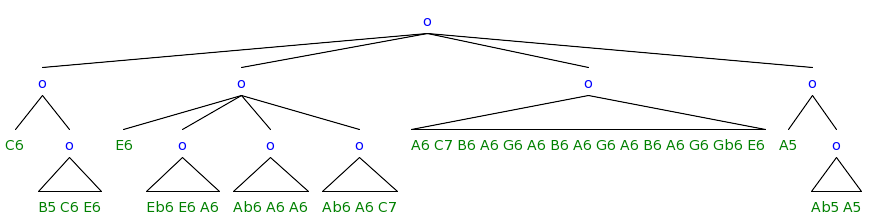
\includegraphics[scale=0.4]{img/onset_sym}
\label{fig:subfig1}
}

\subfigure[Second order delta pitch tree]{
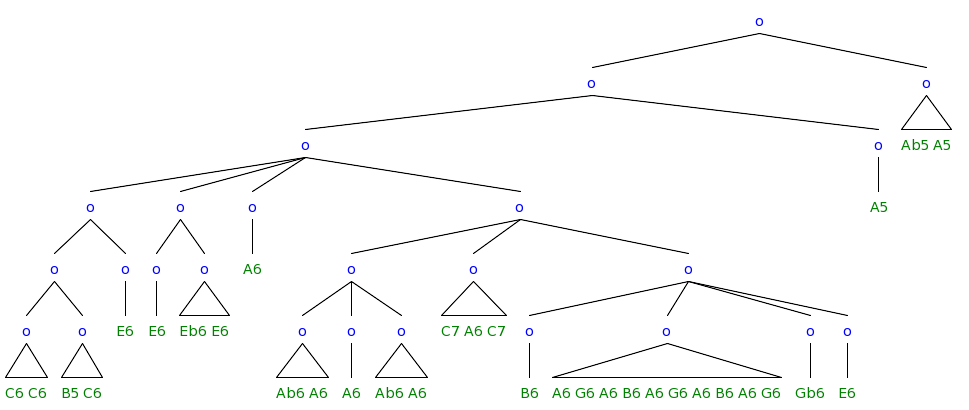
\includegraphics[scale=0.3]{img/second_order_pitch_sym}
\label{fig:subfig2}
}
\caption{Parse trees of the first eight bars of piano sonata KV331 III. (Turkisch March)by Mozart }
\label{fig:pitchonsettrees}
\end{figure}

A delta onset tree and a second order delta pitch tree of the first eight bars of Mozart's Turkish March can be found in figure \ref{fig:pitchonsettrees}. In this figure we can see that some nodes contain only other nodes, some nodes contain only notes and some nodes are mixed and contain notes and other nodes. We will use this differentiation between node types in the translation of a tree into a segmentation, which is shown in algorithm \ref{alg:segmentation}. The algorithm is initialized with the root node.
\begin{algorithm}
\caption{Segmentation}
\label{alg:segmentation}
For some node $n$, do:
\begin{enumerate}
\item \textbf{If} $n$ is a note.\\
\textbf{Then} add $n$ as a singleton segment to the segmentation.\\
 \textbf{Else} expand $n$.
\item \textbf{If} $n$ is mixed and directly contains more than $x$ notes.\\
\textbf{Then} add all notes recursively contained by $n$ as a segment to the segmentation.\\
\textbf{Else} start from step 1 for every child of $n$.
% If $n$ contains at least $x$ notes, add the notes recursively contained by $n$ to the segmentation.
\end{enumerate}
\end{algorithm}

The value of $x$ represents the tolerance of singleton segments. We need this parameter because, in the delta onset tree, very long notes cause one note to split of a constituent at a high level, in this case we want to accept that this one note will be a singleton segment. We have found that setting $x$ to a variable number, namely: the number of notes recursively contained (yielded) by the current node divided by 16 works quite well for works by Mozart. Our segmentation of the first eight bars of Mozart's Turkish March using a delta onset tree can be found in figure \ref{fig:mozartsegments}.\footnote{Note that if the delta tree from figure  \ref{fig:subfig2} is used the segmentation will be different. This segmentation was based on an onset delta tree over the entire piece instead of just the first eight bars.}

%To translate a delta tree into a segmentation we simply take all the nodes at a particular level and consider the notes it yields as one group. However, as can be seen in figure \ref{pitchonsettrees} the trees are quite deep and it is not clear what level we should choose. We can make the trees shallower by slightly modifying the delta rule. We introduce a small tolerance parameter $\epsilon$ and instead of looking for the maximum in of a list of deltas, we look for deltas within $m - \epsilon$ and $m + \epsilon$, where $m$ is the maximum delta within a list of deltas.

%Using this modification of the delta rule we can bring the delta onset tree down to a shallow tree in which it is safe to choose groupings defined by the first level nodes. 


For some works, like most works by Mozart, using only a delta onset tree works very well. However, for other, like Bach's Inventionen, a delta onset tree is not sufficient since the music contains almost no differentiation in IOI (most notes are equidistant in onset).

To overcome this problem we will use pitch. Even though Bach's Inventionen use almost no differentiation in IOI they can be segmented nonetheless. We will not make any attempt to combine pitch interval trees and IOI trees. Instead we take the segmentation given by the IOI tree and try to subdivide every segment using a pitch interval tree. 

The sort of changes in pitch that indicate constituent transitions are not characterized very well by a first-order pitch interval tree. Let us take the example from the previous section, where we have a melody of eight notes, four of which are chromatically ascending followed by four notes that have octave intervals between. We want this to be segmented into two constituents where one contains the four ascending notes and another one contains the notes with octave intervals. A first-order pitch interval tree puts the four ascending notes in one segment but puts the four octave interval notes in four separate segments. A second order pitch interval puts the split in this case exactly where we would want it.

\begin{figure}
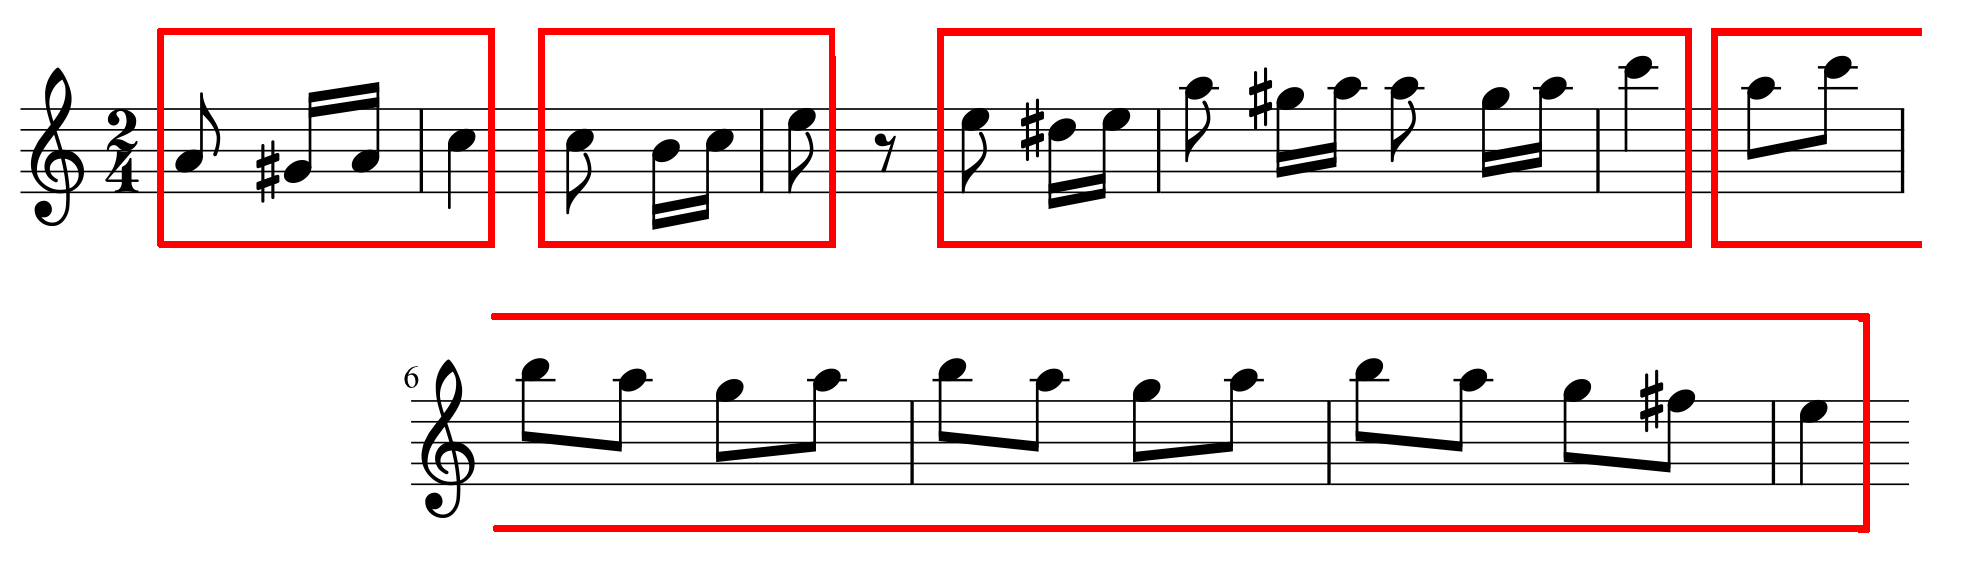
\includegraphics[scale=3]{img/melodysegments}
\caption{First four segments of piano sonata KV331 III by Mozart (grace notes are not shown)}
\label{fig:mozartsegments}
\end{figure}

The pitch interval segmentations are less reliable than the IOI segmentations but since we use pitch only to subdivide IOI segments we can still be sure that some constituent transitions are based on the more reliable IOI segmentation.

\subsection{Constituent Features}
\label{sec:scorefeatures}

We can now convert a piece of music into a series of constituents. These constituents will be used to predict expression, so we must be able to characterize them in a way that correlates with the way they are performed. Analogous to YQX we are looking for the \textit{context} of the constituent, but in contrast to YQX we also need some description of the constituent itself.

YQX uses a set of three score features: pitch interval, duration ratio and I-R arch. The pitch interval is simply the difference in pitch between the current note and the next note. The duration ratio is the logarithmic ratio of the duration of the current note and the duration of the next note.  The I-R arch is is the distance to the nearest point of closure, where closure is calculated from the Implication-Realization analysis \cite{narmour1990analysis}. 

We can generalize pitch interval and duration ratio per note to \textit{context features}: \textbf{mean pitch interval} and \textbf{mean duration ratio}. Definitions can be found below. 
\begin{description}
\item[\textbf{Mean pitch interval}] 
The difference between the average pitch of the current constituent and the average pitch of the next constituent, zero if the current is the last constituent
\item[\textbf{Mean duration ratio}]
The logarithmic ratio between the average note duration of the current constituent and the average note duration of the next constituent
\end{description}

Since I-R arch is related to note-level expression, it does not generalize well to a constituent level feature. 

The two features above provide information about the constituent context: if they are both zero the constituent is apparently similar in mean pitch and mean duration to the next constituent. At note level there is not much to say about the current note besides the pitch and duration. However at constituent level we would also like to say something about the constituent itself. For this purpose the \textit{constituent features} \textbf{mean delta pitch} and \textbf{mean delta duration} are used. These features say something about the amount change in pitch and the amount of change in note duration:
\begin{description}
\item[\textbf{Mean delta pitch}] The average of all absolute pitch intervals within one constituent. 
\item[\textbf{Mean delta duration}] The average of all absolute differences in duration of succeeding notes within one constituent
\end{description}

Note the difference between these features and the context features. The context features use the mean pitch of one constituent and the mean duration within constituent and compare these to the mean pitch and mean duration of the next constituent. The constituent features use the average of all pitch intervals within one constituent and the average of all differences in duration within one constituent, giving a measure of the spread of pitch and differentiation of rhythm within the constituent.

The complete set of score features consists of the two context features and the two constituent features. 

The system does not make use of expressive markings in the score. A mature performance rendering system should incorporate these in some way. Even a human performer is not expected to read the mind of the composer and uses the expressive markings to guide his performance. Disregarding articulation marks and dynamic markings has a significant impact on the results: the system has an overall slight preference for playing staccato and softly. This is due to the fact that staccato notes or notes that should be played soft are treated as normal notes and bias the statistics. 



\subsection{Expression Parameters}
\label{sec:targets}

Every constituent will be assigned expression parameters that indicate how the constituent is played expressively in a performance. These parameters define what we mean by structure level expression and should therefore be chosen carefully. 

Some concepts that we think fall under structure level expression are \textit{crescendo} or \textit{decrescendo}, \textit{ritardando} and \textit{piano} or \textit{forte} etc.
From these, concepts like crescendo, decrescendo and ritardando arguably fall under note level expression and for simplicity we will not consider them structure level expression. In fact, we will only look at the mean tempo, the mean articulation and the mean loudness of a constituent.

YQX defines expression per note in three parameters: \textit{IOI ratio}, \textit{articulation} and \textit{loudness}. These parameters are defined as the logarithmic ratio between the performance IOI and the IOI notated in the score (calculated using some base tempo), the silence after a score note divided by the silence after the performed note and the logarithmic ratio between the loudness of the performed note and the mean loudness of the performance. 

We are going to define our own expression parameters in a similar way, but let us first look at some issues with the definitions YQX uses. The definition of articulations seems to be a bit awkward and inconsistent. Awkward because if a score note is not followed by a rest, the notated silence after it is zero, rendering articulation undefined. Inconsistent because all the other expression parameters use logarithmic ratios and we see no reason not to use a logarithmic ratio for articulation as well. 

IOI ratio and loudness are defined relative to mean performance tempo and loudness. However, to capture micro expression in the form of small changes in onset relative to the beat, it seems more logical to define this feature relative to the local tempo, instead of relative to the global tempo. The same argument can be made for defining loudness relative to local loudness instead of global loudness. Structure level expression may help to define the concepts of local tempo and local loudness as we can simply take the mean tempo and loudness within one constituent and take this to be the local tempo and loudness. See section .

The expression parameters that we will use are:
\begin{description}
\item[Mean Tempo Ratio] The logarithmic ratio between the mean tempo within the constituent and the base tempo of the performance.
\item[Mean Articulation] The logarithmic ratio between performance IOI and the score IOI if the next note is not a rest. If the next note is a rest we use the note duration calculated with the score duration of the note and the local expressive tempo instead of the performance IOI. IOI is the onset of the next note minus the onset of the current note.
\item[Mean Loudness Ratio] The logarithmic ratio of the mean loudness within the constituent and the base loudness of the performance
\end{description}

Admittedly, we still use mean loudness and tempo to calculate tempo and loudness ratio. This is a limitation inherent to using a segmentation instead of hierarchical structure. When using hierarchical structure, the parameters could be defined relative to the parent constituent.

\subsection{Model}
\label{sec:model}


We can now reduce a piece of music, represented as a sequence of notes $M_{i,j}$, of which we have a score and a performance, to a sequence of \textit{score feature vectors} $F$ and \textit{expression parameter vectors} $E$. First, we segment the score into constituents:

\[\mbox{segment}(M_{ij}) = \{c_1, c_2, \cdots, c_n\}\]
We can then extract feature and parameter values from the score and the performance:
\begin{align*}
f_i &= (p_i, d_i, \Delta p_i, \Delta d_i)^T\\
F &= \{f_1, f_2, \cdots, f_n\}
\end{align*}
where $f_i$ is a feature vector, $p_i$ is the mean pitch interval, $d_i$ is the mean duration ratio, $\Delta p_i$ is the mean delta pitch and $\Delta d_i$ is the mean delta duration.
And the expression parameters: 
\begin{align*}
e_i &= (t_i, a_i, l_i)^T\\
E &= \{e_1, e_2, \cdots, e_n\}
\end{align*}
where $e_i$ is a parameter vector, $t_i$ is the mean tempo ratio, $a_i$ is the mean articulation and $l_i$ is the mean loudness ratio.

We can construct a corpus by parsing a number of works in this manner. Given such a corpus, the rendering of a performance can be formulated as maximizing the probability: $P(E|F)$. We can estimate an approximation of this probability by calculating feature likelihoods and transition probabilities. We approximate the features likelihood, which is the conditional probability of a feature vector $f_i$ given an expression vector $e_i$, with the following probability:

\begin{equation}
\label{emission}
P(f_i|e_i) = \frac{c(f_i, e_i)}{c(e_i)}
\end{equation}

Where $c(x)$ is the number of occurrences of $x$ in the corpus.
The expression transition probability is approximated by the unigram count of $e_i$ divided by the bigram count of $e_{i-1}, e_i$.
\begin{equation}
\label{transition}
P(e_i|e_{i-1}) = \frac{c(e_{i-1}, e_i)}{c(e_{i-1})}
\end{equation}
where we make the simplification that expression in one constituent is only dependent on the expression in the previous constituent which is of course not true.

The problem of creating a performance of a score is now reduced to finding a suitable sequence of expression vectors, given a sequence of feature vectors. We can calculate the probability of one expression vector of a performance as the product of the probabilities defined in equations \ref{emission} and \ref{transition}. The probability of the entire performance is approximated by the product of the individual expression vector probabilities.

\[
P(E|F) = \displaystyle\prod_{i=1}^{n}P(f_i|e_i)P(e_i|e_{i-1})
\]

The resulting model is analogous to a stochastic part of speech tagger based on a hidden Markov model where we have substituted words for score feature vectors and parts of speech for expression parameter vectors. Rendering a performance is like finding the most likely part of speech tags for a sequence of words. In our case:

\[E^* = \mbox{argmax}_E P(E|F)\]

which can be found using Viterbi decoding \cite{forney1973viterbi}.

\section{Implementation}
\label{sec:implementation}

This section will discuss practical issues that we faced creating a complete performance rendering system based on the method described in the previous section.

\subsection{Corpus and Representation}
\label{sec:corpus}
We were lucky to find and receive permission to use the CrestMusePEDB \cite{hashida2008new}, which is a database containing expressive performances of Western classical music by famous pianists, including Glenn Gould, Vladimir Horowitz and Maurizio Pollini. The music in this database includes works by Bach, Beethoven and Chopin.

Every performance is accompanied by an XML file containing information on how every note from the score is performed. This information consists of a loudness deviation, attack deviation and release deviation. The loudness is defined relative to a base loudness. The attack and release deviation are defined as the portion of a local beat duration that the attack and release deviates from the score. 

Local tempo is defined for every beat in every measure as the ratio of the tempo in that beat and the base tempo. 

To prepare a score and performance from the database for use in our system we use the score to extract melody notes. We do this simply by taking notes in the highest voice in the top staff. From now on when we talk about pieces and notes we mean melodies and melody notes.

Attack and release are clearly note level parameters so we do not use them. We only need tempo deviations and loudness deviations. The average tempo of a constituent is determined by the average tempo deviation of all the beats that fall within the constituent. The average loudness is determined by the average loudness deviation of every note within the constituent.

The delta functions that are used in the segmentation process use pitch intervals and duration ratios. The pitch intervals use MIDI note numbers which range from 21 to 108 and go up one semi-tone with each step. Durations are in milliseconds, calculated from the score and a standard tempo, set at 120 beats per minute.

We constructed two corpora from the database, one consisting of all performances of Chopin and one consisting of all performances of Mozart in the CresMusePEDB.

\subsection{Discretization}
\label{sec:discretization}

We chose to make the model discrete. We discretize expression and score features in a different way.

\paragraph*{Expression} Discretization of expression parameters is a delicate subject, we want to capture small changes in dynamics and tempo precisely, but outliers may fall in large bins. A sigmoid function is very useful for this purpose. The expression parameters are all logarithmic ratios so they theoretically vary from $-\infty$ to $\infty$. Therefore we first normalize the parameters by dividing it by the minimum absolute value found in the corpus. Discretization of a normalized expression parameter $p$ into $d$ bins is now done as follows:

\[
D(p) = \mbox{floor}\left(\frac{d}{1+e^{-sp}}\right)
\]

Where $D(p)$ is the discretization of $p$, $s$ is a special sensitivity parameter indicating how small the changes in tempo that the discretization captures can be; a larger $s$ means a more sensitive discretization. Undiscretization is the reverse operation:

\[
D^{-1}(p) = s^{-1} d^{-1}(-\log(p^{-1}) - 1)
\]

\paragraph*{Features}

To discretize the features, we simply normalize every feature dividing through the maximum absolute value of that feature found in the corpus. After normalization we multiply the feature by a discretization parameter $d$ that determines the number of bins and take the floor.

\[
D(f) = \mbox{floor}(f*d)
\]

Where $f$ is the normalized feature value.

\subsection{Smoothing}
\label{sec:smoothing}

Despite having discretized our feature and observation vectors we often find that we observe feature vectors in a new score that we had never seen during training. We do not want the conditional probabilities from equation \ref{emission} to become zero so we have to smooth these probabilities. We use a smoothing technique known as simple Good-Turing smoothing \cite{gale1995good}. The idea is that we use the probabilities of things we have seen once for the things we have never seen. Recall how we calculate the conditional probability of a feature vector:

\[
P(f_i|e_i) = \frac{c(f_i, e_i)}{c(e_i)}
\]

Let us call the $c(f_i, e_i)$ the coincidence count. Let $N_c$ be the number of things with frequency $c$ in the corpus. For example if there are five coincidences $(f_x, e_x)$ nd no other pair of $f$ and $e$ occurs five times, then $N_{5} = 20$. Good-Turing re-estimates counts according to this formula:

\begin{equation}
\label{count}
c^* = (c+1) \frac{N_{c+1}}{N_c}
\end{equation}

The smoothed probability of some event $x$ is

\[P(x) = \frac{c^*}{N}\]

In our case, the probability we seek is $P(f_i|e_i)$, the sample size $N$ is therefore the number of times we have seen $e_i$: $c(e_i)$. $N_c$ is the number of coincidences with $e_i$ that we have seen $c$ times. The count $c$ is $c(f_i, e_i)$ and $c^*$ is derived using equation \ref{count}. The 

\[P(f_i|e_i) = \frac{c^*}{c(e_i)} \mbox{ for all } c > 0 \]

By applying this formula to all counts larger than zero we reserve approximately $\frac{N_1}{N}$ probability mass for things that we have never seen. We assign an equal probability for all unseen feature vectors, namely:
\[
P(f_{\mbox{unseen}}|e_i) = \frac{1}{U} \frac{N_1}{c(e_i)} 
\]
Where U is the number of unseen coincidences, which is determined by the number of different observations in the corpus plus the new observations from the score minus the number of coincidences with $e_i$.

In order to make this work we cannot use $N_c$ directly since it will not be defined for every $c$. We use a least square approximation to the following function. 

\[\log(N_c) = a + b \log(c)\]

This completes the definition of simple Good-Turing smoothing. However, even now there may still be some expression parameter vectors that occur with only unique feature vectors, so that for that expression only $N_1$ is defined. We cannot fit a function to one sample, so if we have only one $N_c$ sample, we simply turn off Good-Turing smoothing and accept the fact that some probabilities will be zero. 

In practice we have to use quite a large bin size. Despite this large bin size, many combinations of features and expression parameters were never encountered during training. The same applies to transitions of expression: only small portion of all possible transitions of expression are actually encountered in the corpus. Some of the feature likelihoods can be smoothed like we described above, but the transition probabilities are not smoothed at all. Since our model does not allow zero probability transitions (this would make the likelihood of the entire performance zero), our model is heavily overfitting. The resulting performances only contain changes of expression that were actually encountered in the corpus.

In most applications of machine learning, this degree of overfitting would not be acceptable. However, in this particular application we seem to be able to get away with it. Playing phrase transitions exactly as encountered in the corpus seems to be acceptable as long as we play the right transitions at the right moment. The overfitting and the large bins size gives the performances a bit of a stereotypical and cartoonistic feel. A larger corpus allows would reduce the overfitting and the requirement of large bins, but this kind of corpus is not available to us at the moment.

\subsection{Performance rendering}

Our model is able to generate expressively performed melodies but does not handle polyphony. During training, the bass and harmony notes were stripped off. After rendering an expressive performance we can simply put them back in and estimate their expressive parameters. We do this by giving each bass and harmony note the expressive parameters of the last played melody note. 

Unfortunately the notes we treat as melody notes are not always the notes that humans perceive as melody notes. Sometimes the melody is voices other than the top voice. In other cases, like Bach's fugues, there are multiple melodies in multiple voices at the same time. In addition to that, bass and harmony notes should generally not be played with th same expression as melody notes. Bass notes, for example, tend to be played slightly softer and more legato than melody notes.


%\begin{itemize}
%\item Extract melody
%\item Extract score features from melody
%\item lookup notes in deviation, ignore missing notes
%\item Extract expressive and non-expressive melody and extract expression features
%\item Perform notes other than melody notes the same as the nearest melody note
%\end{itemize}

\section{Results}
\label{sec:results}

We compiled two corpora from the CrestMusePEDB. One contained 42 performances of 13 piano works by Mozart, the other contained 49 performances of 19 works by Chopin. We suspect that performances of Mozart's music most outspokenly use structural level expression. Expression within a constituent tends to be more unsteady in performances of Chopin's music. In musical terms, more expression like riterdando, crescendo and rubato is used.

To test the system we trained it on one of the two corpora and let it perform a number of works. Here we show the results of four renderings of Chopin's Mazurka No. 19, Op. 30-2 and Mozart's Piano Sonata 310 III. To see what the effect was of each corpus on different styles of music we performed each work on both corpora. For reference, we also show a performance by a real human pianist that was used during training. Given the small dataset and the free nature of expression we did not expect the performances to correlate much with performances by human pianists and as can be seen in the results they indeed do not. 

For all four performances the system was trained with a discretization factor of five. In practice, this means that the constituent features (see section \ref{sec:scorefeatures}) were discretized into five bins and the context features into a slightly larger number of bins since their values can be negative as well. The expression features were discretized into ten bins, with a sensitivity of five. The bins had to be this large to recognize most of the score features in the score that was to be performed. 

Segmentation was done using only delta onset trees. This proved to be most reliable for Mozart and Chopin. 

When rendering a Mozart performance on the Mozart corpus and a Chopin performance on the Chopin corpus all performances of the piece that had to be performed were left out of the corpus during training. 

Plots showing dynamics, tempo and articulation of the resulting performances are shown in figure \ref{fig:mozartperformances} and \ref{fig:chopinperformances}.\footnote{Of course, staring at plots of music performances is not nearly as informative as actually listening to them. For this purpose, a few performances including the ones shown here can be found online at \texttt{http://soundcloud.com/expressiveperformance/sets/final-results/}.} The values on the y-axis, labeled deviation, are the exponents of the expression parameters, which themselves are logarithmic ratios. In other words, the values indicated by the axes are ratios. A tempo of $2.0$ means twice as fast as the average tempo, an articulation of $0.5$ means the notes are played twice as short as notated in the score, a dynamic value of $0.5$ means the notes are played half as loud as the average loudness of the performances. Likewise, to translate the output of the system into a performance, the mean tempo and loudness have to be set manually. 

The performances are plotted per note. The block like character of the axes is caused by the segmentation. For the sake of comparison, the performances by human pianists have been averaged over each constituent and discretized, so these plots show how the performance is represented in the corpus.


%The system was tested on works from Mozart as we do not expect our system to generalize well to other composers.  We used

\begin{figure}
\centering

\subfigure[Performance by the system trained on the Mozart corpus]{
\includegraphics[scale=0.4]{img/Mozart-snt310-3_MozartNewSegmentation2_legend}
\label{fig:donset}
}

\subfigure[Performance by the system trained on the Chopin corpus]{
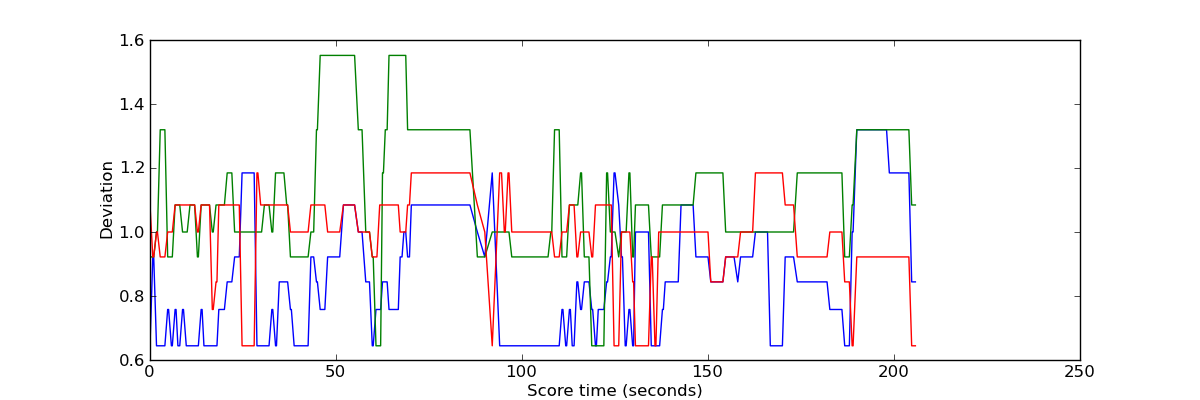
\includegraphics[scale=0.4]{img/Mozart-snt310-3_ChopinNewSegmentation}
\label{fig:donset}
}

\subfigure[Performance by Maria Jo\~ao Pires]{
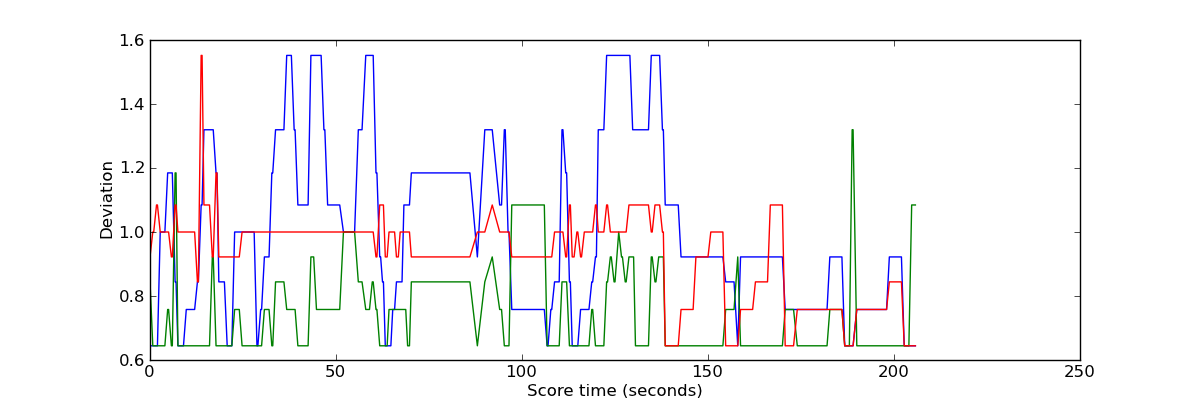
\includegraphics[scale=0.4]{img/Mozart-snt310-3_pires}
\label{fig:donset}
}
\caption{Three performances of Mozart's Piano Sonata 310 III.}
\label{fig:mozartperformances}
\end{figure}

\begin{figure}
\centering
\subfigure[Performance by the system trained on the Mozart corpus]{
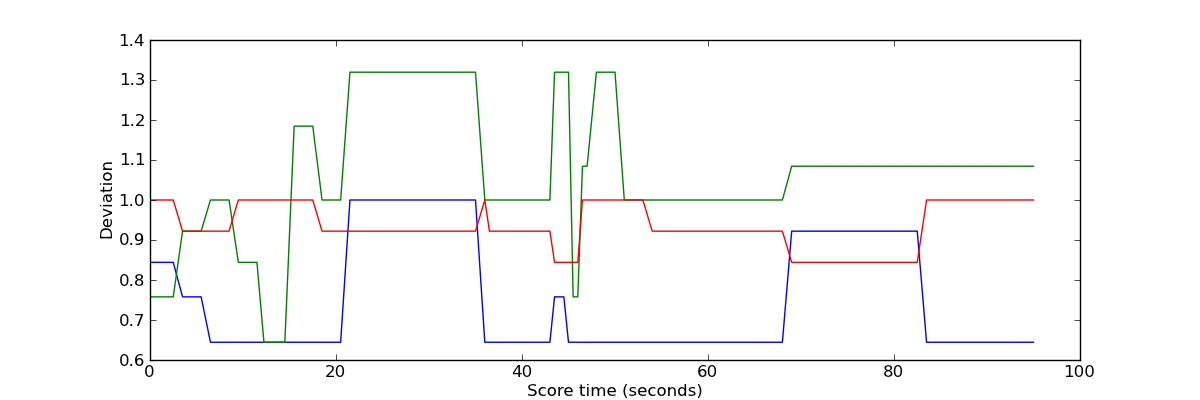
\includegraphics[scale=0.4]{img/Chopin-mzk019_MozartNewSegmentation2}
\label{fig:donset}
}
\subfigure[Performance by the system trained on the Chopin corpus]{
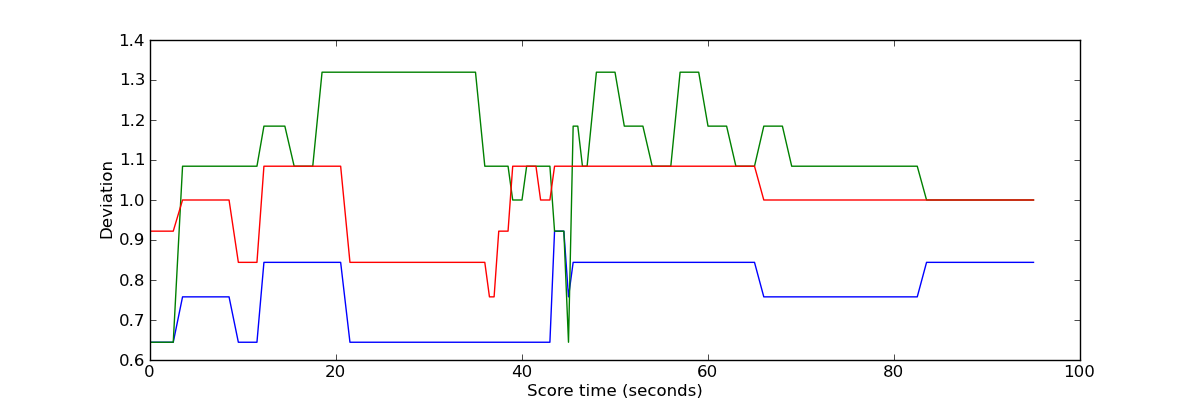
\includegraphics[scale=0.4]{img/Chopin-mzk019_ChopinNewSegmentation}
\label{fig:donset}
}
\subfigure[Performance by Samson Francois]{
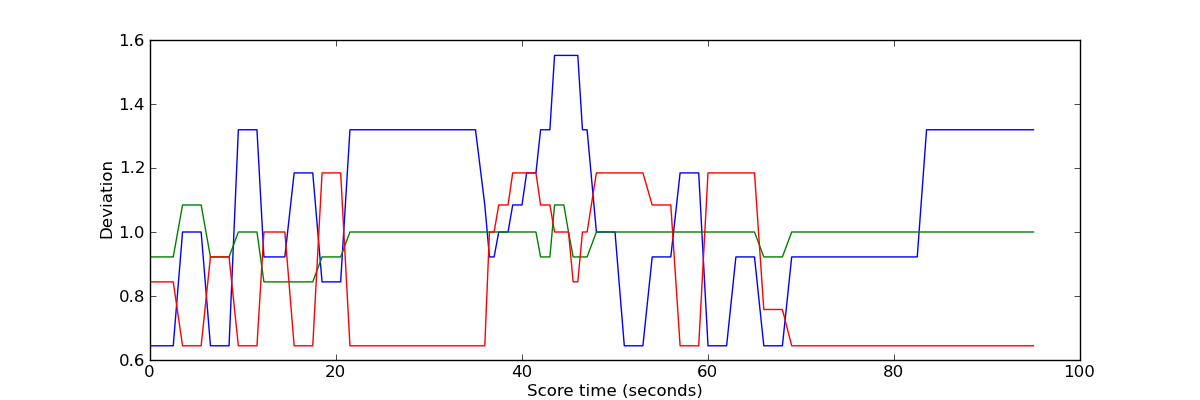
\includegraphics[scale=0.4]{img/Chopin-mzk019_franc}
\label{fig:donset}
}
\caption{Three performances of Chopin's Mazurka No. 19, Op. 30-2}
\label{fig:chopinperformances}
\end{figure}



\section{Discussion and Evaluation}
\label{sec:discussion}

%. Whether it makes musical sense to perform Chopin on a system trained on Mozart is left for the reader to decide. 
In the introduction, we mentioned the problem of evaluation. The most effective evaluation that is available at the moment is participation in the performance rendering contest, Rencon \cite{hiraga2002rencon}. Unfortunately, participating in this contest was not feasible for this project. Therefore we are left with our own subjective observations and qualifications. 


% Phrase transitions
% Qualitative judgements
% Comparison
% Segmentation

When listening to the performances generated by our system, the effect of per-segment expression can clearly be heard. Making changes in dynamics at phrase transitions effectively increases the human feel of a performance. These dynamics changes work well when phrase transitions are correctly detected. Sometimes however, when a phrase transition is incorrectly detected, changes in dynamics can be very disrupting. This can be heard in the system's rendering of Mozart's Piano Sonata KV331 I. when trained on the Chopin corpus. At the end of the second bar, a transition is detected one note too early, causing a strong accent to be placed at an uncomfortable point in the piece. These incorrectly detected transitions are not systematic and in general the transitions detected by the system are musically plausible, if not, interesting.

Changes in tempo are riskier than changes in dynamics. Small changes in dynamics, when made at phrase transitions at least, do not disrupt a performance as much as small changes in tempo at the wrong moment. Often, the tempo deviations the system makes sound good or at least acceptable, but the system does tend to sometimes produce awkward sounding changes in tempo, like a sudden slow down that can be heard a number of times in our results online.

Despite the fact that our system only determines expression per segment, small segments and gradual changes in dynamics or tempo can give a crescendo or accelerando feel to certain parts of the music. It was interesting to see that this could be achieved using only structure level expression.

The system clearly accentuates structure, but only on the level of the segmentation. Although locally the changes in dynamics, articulation and tempo often seem sensible, at a higher level there does not seem to be an idea behind it all and the overall flow of the performance seems a bit random. When theme is repeated a few times, the system may perform it completely different each time. While some variation when playing a repetition of a phrase makes a performance interesting, playing it completely different each time conveys the feeling that the performer does not really know what he is doing. This sort of randomness comes as no surprise since our model uses only transition probabilities and local expression probabilities. To really capture global flow of performance, a grasp of hierarchical structure and repetition seems crucial.

Ignoring note level expression has been an adequate way to demonstrate the phenomenon of structure level expression. Yet, we cannot deny the need for note level expression in a performance rendering system that intends to completely simulate human expression. Section \ref{sec:futurework} suggests a possible integration of structure and note level performance rendering systems.


\section{Conclusion}
\label{sec:conclusion}

In this thesis, we have introduced a way of recognizing and using structure level expression. We argued why we think it is a crucial aspect of performance rendering systems and we criticized  note level performance rendering for not being able to correctly learn to make daring and large changes in expression as well as lacking the ability to convey structure level expression. 

Our goal was to create a system that, in contrast to a note level performance rendering system, dares to make sudden big changes in expression and clearly accentuates musical structure. Our results show that our system indeed is not shy about this kind of big expressive changes. The performances of the system contain sometimes smooth, sometimes sudden changes of expression that really do seem to be an improvement over note level performance rendering systems.% It is up to the listener to judge whether these changes are actually an improvement over the smoother performances of note level performance rendering systems.

The system that we proposed reduces the idea of structure to a segmentation of a score into constituents based on a structural analysis. For the structural analysis, we used the delta framework \cite{markwin}, proposed by Markwin van den Berg. We noticed that a segmentation based on onset delta trees works well for some music but does not recognize all constituent transitions. To overcome this we suggested to use a second order pitch delta tree, but we ended up discarding this idea because it produced too many incorrect splits in phrases. Our system would therefore not work very well on music that has a consistent rhythmic structure like some of Bach's music. In the end, an onset tree segmentation worked well enough to produce musically relevant segmentations given the right genre of music.

To characterize constituents and their relations to other constituents we used constituent likelihoods and bigram transition probabilities of expression. The resulting hidden Markov model could be used in combination with Viterbi decoding to generate performances. This approach is very similar to stochastic part of speech tagging using hidden Markov models.

\section{Future Work}
\label{sec:futurework}

%Clearly, performance rendering systems do not come close to the expressiveness of real human performances. 
We have presented a new approach to performance rendering, one that is purely structure based. Our first results look promising but also clearly demonstrate some limitations of our system. We think that these limitations are easily identifiable and addressed and with some extensions, structure based performance rendering can bring us far. We will shortly list some of the limitations that we discussed in our evaluation in section \ref{sec:discussion} and provide some suggestions on how to address them.

The segmentation of a score is not always perfect and leaves room for improvement. Ultimately, we do not want discard the idea of a segmentation completely and move to a multilevel structure analysis, this will help to eliminate the randomness that we discussed in our evaluation. Whether the delta framework can be used for such an analysis remains a topic for future research. The delta framework offers us more analytic power than we have used in this system. But in order to use it to generate multilevel structure, a way to combine different delta trees into one consensus tree is needed.

Another open problem is how we should deal with multiple voices. Some proposals have been made in this field. Tae Hun Kim et al. \cite{kim2010performance} split a piece into melody, bass and harmony and use separate probabilistic models for each of them. When using different expression for different voices, another problem presents itself, namely how to synchronize the voices so that the performance still sounds like it is played by one performer or a group of performers with an adequate mastery of timing. Pop-e \cite{hashida2006pop} uses an automatic analysis to determine the attentive part in music: the voice of the music perceived as melody at any point in the piece. It uses this information to synchronize expression in different voices.

As we mentioned in our evaluation, our system ignores expressive markings. The result is that depending on the corpus, the performance renderer has unwanted biases. A possible approach to incorporating expressive markings in the system is to determine what, given an expressive mark in the score, is the average way to play a given note and normalize this out of the corpus. Say staccato notes are played, on average, half length notated in the score, we specify articulation deviation relative to this half duration instead of the full duration. That way the system now recognizes the note as a normal staccato note instead of an extremely short legato note. 

We hope that in the future, as the CrestMusePEDB project develops, data sparsity will be less of a problem. For now however, we are left with having to do discretization and smoothing. The smoothing technique we used, Good-Turing smoothing, is arguably not the best way to smooth the corpus. Good-Turing smoothing assigns equal probabilities to all unseen score features. It is likely that unseen score features that are very similar to score features that we have seen should also be played in a similar way as the score features they resemble. A different smoothing technique may be able to use this information. We could use a smoothing technique similar to Katz-Backoff \cite{katz1987estimation}: Upon encountering an unseen feature vector, discretize again the corpus into increasingly larger bins until we do find the feature vector in our corpus.

% where the frequency of an N-gram with zero occurrences is approximated by backing off to the count of the (N-1)-grams, (N-2)-grams, etc. until the count is not zero anymore. 

The system would certainly benefit from a notion of repetition and similarity. Repetition is a very good indicator of constituent breaks. Repetition and similarity could also be used to improve expressiveness of performances. It is probably telling when a phrase is repeated three times and then slightly altered the fourth time. Although finding similarity and musically significant repetition is a subject of its own, the delta framework could help to define repetition arbitrarily of transposition or rhythm. A list of pitch deltas can for example be used to detect repetition independent of transposition and a list of duration deltas can be used to detect repetition of rhythm independent of the notes used. 

The YQX system defines expressive tempo implicitly by predicting the logarithmic ratio of the IOI in a performance and the IOI in a score. Timing alterations of notes are always defined relative to the base tempo. This does not correspond to the intuition that the \textit{the tempo itself} is altered during the performance, resulting in a local tempo, and that rhythmic changes should be seen relative to this local tempo. The same applies to the way YQX looks at loudness. This is specified as the logarithmic ratio between the notes loudness and the mean loudness of the performance. 

An integration of constituent level expression and note level expression can provide a solution to this problem. We can define expressive tempo relative and dynamics relative to the expression parameters of the constituent. A possible approach is to first define constituent level expression and use a note level expression system on each constituent separately.

As we mentioned in section \ref{sec:approach} the ability of the system to characterize constituents and their relations to other constituents in a musically relevant way is an important factor influencing the results. We do not have the illusion that a set of four score features and bigram transition probabilities are a valid model of human musical intuition, let alone producing highly expressive performances. A better notion of repetition, a notion of key, harmony and general musical knowledge are the least that seems to be required for that purpose.

Finally we would like to make a small comment about the possible value of performance rendering in an artistic sense. Computer generated performance, and in a broader view, computer generated art, is often criticized for merely copying a very specific human behavior and not really contributing something new. We think a very small hint at the way computer generated performances may one day be able to provide a really new perspective on music performance, is given by our system: when listening to the performances of the systems we noticed sometimes the system made surprising phrase transitions or suggested a phrase transition at a surprising point in the music. Surprising, because no pianist would probably think about making these expressive decisions, yet they did not sound bad, making the performance truly unique. This closing note gives us hope that the field of computer generated performances not only copies human performances but humans may one day learn from computer generated performances.

%\section{Acknowledgements}

%I would like to thank Remco Scha for providing guidance and support. I am very grateful to the CrestMusePEDB project for kindly providing me access to their database that they have p
\pagebreak
 \bibliographystyle{plain} % plain, nature, jbact
 \bibliography{myref} 

%\appendix
%\section{Corpus}
%\label{appendix:corpus}
%\begin{tabular}{ll}
%\textbf{Work} & \textbf{Performer}\\
%\hline
%Sonata KV331 \MakeUppercase{\romannumeral 1}. & Hiroko Nakamura\\
%& Glenn Gould\\
%& Christoph Eschenbach\\
%& Ingrid Haebler\\
%& Lili Kraus\\
%& Maria Jo\~ao Pires\\
%& Alicia De Larrocha\\
%& kn?\\
%& yi?\\
%& tn?\\
%& Norio Shimizu\\
%& mo\\
%& mk?\\
%& ea?\\
%& nm?\\
%& kt?\\
%& tm?\\
%\hline
%Sonata KV331 \MakeUppercase{\romannumeral 2}. & Hiroko Nakamura\\
%& Maria Jo\~ao Pires\\
%& Alicia De Larrocha\\
%& ea?\\
%\hline
%Sonata KV331 \MakeUppercase{\romannumeral 3}. & Hiroko Nakamura\\
%& Maria Jo\~ao Pires\\
%& Christoph Eschenbach\\
%\hline
%Sonata KV545 \MakeUppercase{\romannumeral 1}. & Maria Jo\~ao Pires\\
%& Glenn Gould\\
%\hline
%Sonata KV545 \MakeUppercase{\romannumeral 2}. & Maria Jo\~ao Pires\\
%& Glenn Gould\\
%\hline
%Sonata KV545 \MakeUppercase{\romannumeral 3}. & Maria Jo\~ao Pires\\
%& Glenn Gould\\
%\hline
%Sonata KV279 \MakeUppercase{\romannumeral 1}. & Glenn Gould\\
%& Maria Jo\~ao Pires\\
%\hline
%Sonata KV279 \MakeUppercase{\romannumeral 2}. & Glenn Gould\\
%& Maria Jo\~ao Pires\\
%\hline
%Sonata KV279 \MakeUppercase{\romannumeral 3}. & Glenn Gould\\
%& Maria Jo\~ao Pires\\
%\hline
%Sonata KV310 \MakeUppercase{\romannumeral 1}. & Maria Jo\~ao Pires\\
%& Glenn Gould\\
%& Hiroko Nakamura\\
%Sonata KV310 \MakeUppercase{\romannumeral 2}. & Maria Jo\~ao Pires\\
%Sonata KV310 \MakeUppercase{\romannumeral 3}. & Maria Jo\~ao Pires\\
%Sonata KV570 \MakeUppercase{\romannumeral 3}. & nm?\\
%\end{tabular}




 
 
\end{document}
